\documentclass[11pt]{article}
\usepackage[T1]{fontenc}
\usepackage[margin=1in]{geometry}
\usepackage{amsmath,amssymb,amsthm}
\usepackage{graphicx}
\usepackage[colorlinks=true,linkcolor=blue,citecolor=blue,urlcolor=blue]{hyperref}
\theoremstyle{remark}
\newtheorem{remark}{Remark}[section]
\newcommand{\Tr}{\operatorname{Tr}}
\newcommand{\deff}{d_{\rm eff}}

\title{Operational Signatures of Criticality from Petz Recovery\\
{\large Collar-length requirements in TFIM exact diagonalization}\\
{\normalsize Version 2}}
\author{Lluis Eriksson\\ Independent Researcher\\ \texttt{lluiseriksson@gmail.com}}
\date{January 2026 (v1); July 2026 (v2)}

\begin{document}
\maketitle

\begin{abstract}
We study whether recovery-based operational distances exhibit a distinctive
finite-size signature near quantum criticality. For a tripartition
$A$--$B$--$C$ of a 1D chain with a collar $B$ of width $w$ separating $A$
from $C$, we compute a Petz-based reconstructed state and the recovery
error $E_{\rm Petz}(w) = -\log F$ (squared Uhlmann fidelity), and define an
effective recovery distance $\deff(\varepsilon)$ as the minimal collar
width achieving error below $\varepsilon$, stabilized by $E_{\rm best}(w)
= \min_{w' \le w} E_{\rm Petz}(w')$ and reported with explicit censoring.
Using exact diagonalization of the transverse-field Ising chain at
$N = 11$ with $|A| = 2$, we sweep $h_x$ across the critical region at
$h_z = 0$ and compare to a longitudinally perturbed control $h_z = 0.5$:
pronounced growth and extensive censoring of $\deff(\varepsilon)$ appear
in the critical region at low temperature, while the control remains
comparatively featureless; an extended-collar spot-check yields
$\deff(10^{-3}) \approx 7.6$--$7.7$ at $\beta = 12$ near $h_x \in \{0.96,
1.00\}$. \emph{v2 adds (no v1 result is changed):} an explicit
$|C|$-shrinkage caveat -- at fixed $N$, growing $w$ also shrinks $C$, so
the \emph{absolute} scale of $\deff$ near $w_{\max}$ conflates buffer
growth with a shrinking reconstruction target, while fixed-geometry
comparisons across $h_x$ (the criticality signature) are unaffected; a
window-relativity remark ($\varepsilon$, $\beta$, $N$ jointly set what is
resolvable: at smaller $N$ the $\beta = 12$, $\varepsilon = 10^{-3}$
window censors even off-critical points, consistent with v1's own zoom);
delivery of v1's ``future work'' item: a CMI-based distance computed on
the same sweep shows the \emph{same} criticality signature at its own
threshold (CMI decays about half as fast as the Petz error, cf.\
2601.0035); series positioning; and a fully regenerable verification
suite.
\end{abstract}

\section{Introduction}
Approximate quantum state recovery provides an operational way to quantify
how much information about a subsystem can be reconstructed from a
surrounding collar. We test whether recovery performance exhibits a
characteristic finite-size signature when a lattice model is tuned through
a quantum critical region. We do not claim a thermodynamic divergence at
finite size: the object is a finite-$N$, finite-$\beta$ diagnostic --
whether the collar length required for a fixed recovery threshold grows
sharply near the expected critical point and differs from an explicitly
perturbed control.

\paragraph{Series positioning (added in v2).} This note extends the
non-Gaussian recovery block of the series to criticality: the ED pipeline,
model family and censored-fit discipline are those of 2601.0035
\cite{S0035} (whose corrected FR scale also calibrates how to read
$-\log F$ against CMI); the crossover-width diagnostic $w^*$ of 2512.0101
v2 \cite{S0101} is the cousin of $\deff$; the upstream program is
2512.0060 \cite{S0060} with Type III capstone 2601.0034 \cite{S0034}.

\section{Setup and definitions}
As in v1: $E_{\rm Petz}(w) := -\log F(\rho_{ABC},
\tilde\rho^{\rm Petz}_{ABC}(w))$ with $F(\rho,\sigma) =
(\Tr\sqrt{\sqrt\rho\,\sigma\sqrt\rho})^2$; $E_{\rm best}(w) :=
\min_{w'\le w} E_{\rm Petz}(w')$; $\deff(\varepsilon) := \min\{w :
E_{\rm best}(w) \le \varepsilon\}$ with log-linear interpolation;
censoring $\deff(\varepsilon) > w_{\max}$ reported explicitly, always
against the \emph{effective} $w_{\max}$ actually evaluated.

\begin{remark}[$|C|$-shrinkage caveat (added in v2)]
\label{rem:cshrink}
At fixed $N$ and $|A|$, increasing $w$ necessarily shrinks $|C| = N - |A|
- w$: at the extended-collar spot-check values $w = 7, 8$ with $N = 11$,
the reconstruction target $C$ has only $2, 1$ sites. Reconstructing a
smaller $C$ is intrinsically easier, so the \emph{absolute} reading
``operational recovery length $\approx 8$ sites'' conflates genuine
buffer-length requirements with a shrinking target and should be treated
as an upper-bound-flavored diagnostic at this system size. The
\emph{signature} claims are unaffected: all critical vs off-critical vs
control comparisons are made at fixed $(N, |A|, w)$ geometry, where $|C|$
is identical across the compared points. A fixed-$|C|$ protocol (growing
$N$ with $w$) is the natural sequel and is listed in the outlook.
\end{remark}

\section{Model and numerics}
As in v1: $H = -J\sum Z_iZ_{i+1} - h_x\sum X_i - h_z\sum Z_i$, open
boundaries, $J = 1$, $h_z \in \{0, 0.5\}$, Gibbs states by ED, $|A| = 2$
at the left edge, coarse sweep $h_x \in [0.7, 1.3]$ and zoom $[0.95,
1.05]$, $\beta \in \{4, 8, 12\}$.

\section{Results}
All v1 results stand unchanged: Figure~\ref{fig:coarse} (coarse sweep:
growth and censoring near $h_x = 1$ at $h_z = 0$, featureless control at
$h_z = 0.5$); the zoom behavior (at $N = 11$: $\beta = 12$,
$\varepsilon = 10^{-3}$ fully censored within $w_{\max} = 7$ across the
zoom window; $\beta = 8$ uncensored; $\varepsilon = 10^{-4}$ censored for
both); and the extended-collar spot-check $\deff(10^{-3}) \approx 7.710$
at $h_x = 0.96$, $\approx 7.627$ at $h_x = 1.00$ ($\beta = 12$, effective
range $w \le 8$; see Remark~\ref{rem:cshrink} for how to read the
absolute value).

\begin{remark}[Window relativity (added in v2)]
\label{rem:window}
What is resolvable depends jointly on $(\varepsilon, \beta, N)$. The
regenerated benchmark at $N = 9$ makes this concrete: at $\beta = 12$,
$\varepsilon = 10^{-3}$, \emph{every} point of the coarse sweep censors,
including far off-critical ones (the off-critical correlation length
already exceeds the accessible window at that threshold and size) --
consistent with v1's own fully-censored zoom at $\beta = 12$. The
critical/off-critical contrast reappears at $\varepsilon = 10^{-2}$:
$\deff = 3, 5, 5, 5, 4, 3$ across $h_x = 0.7, \dots, 1.3$ at $h_z = 0$,
with the $h_z = 0.5$ control flat at $\deff = 1$, and is attenuated at
$\beta = 4$ (flat $\deff = 2$). Signature claims are therefore always
window-relative statements, as v1's finite-$N$/finite-$\beta$ framing
intended.
\end{remark}

\begin{figure}[h]\centering
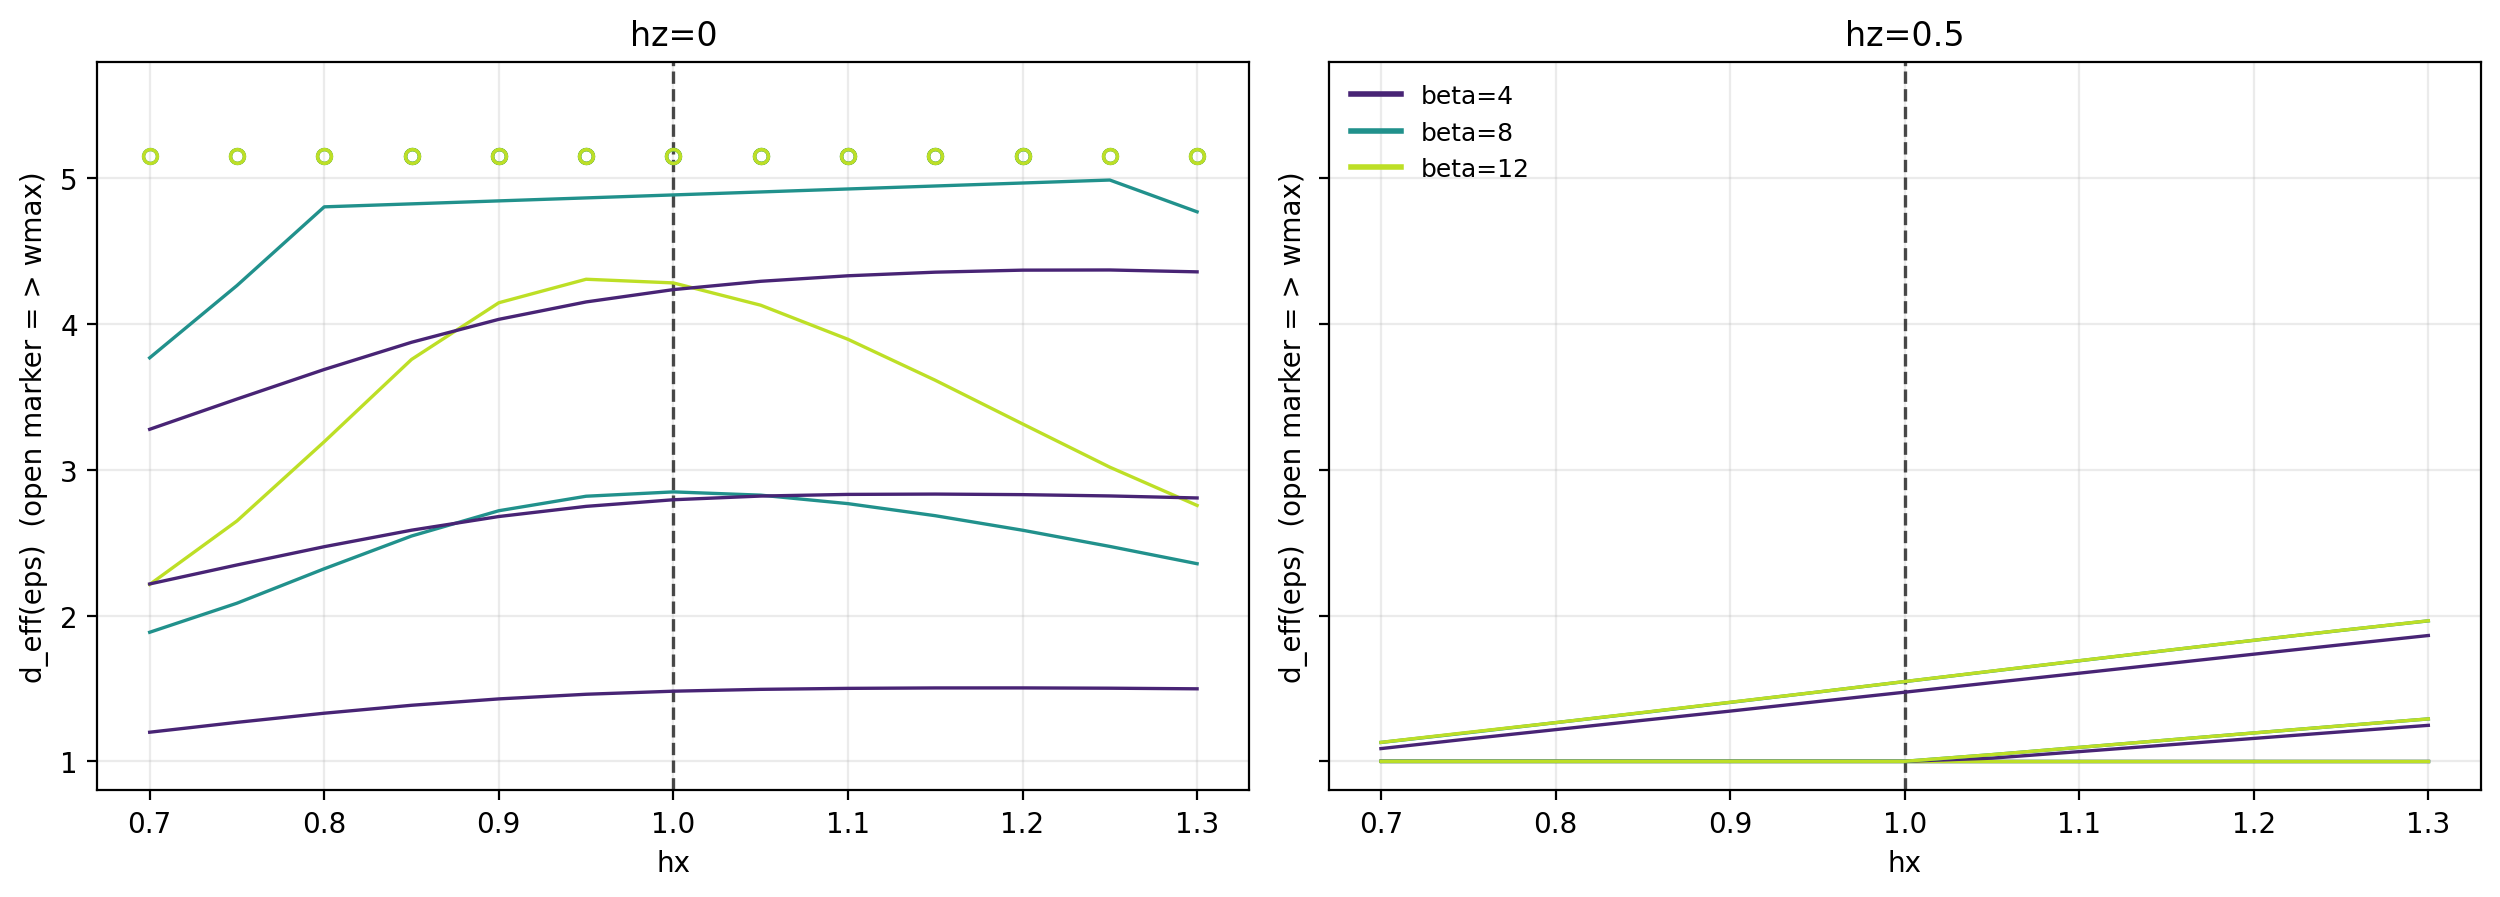
\includegraphics[width=0.95\textwidth]{fig1_coarse_sweep.png}
\caption{Coarse sweep of $\deff(\varepsilon)$ vs $h_x$ for $h_z = 0$ and
$h_z = 0.5$ at $N = 11$, $|A| = 2$ (v1 figure, unchanged). Open markers:
censored ($\deff > w_{\max} = 5$). Dashed line: $h_x = 1$.}
\label{fig:coarse}
\end{figure}
\begin{figure}[h]\centering
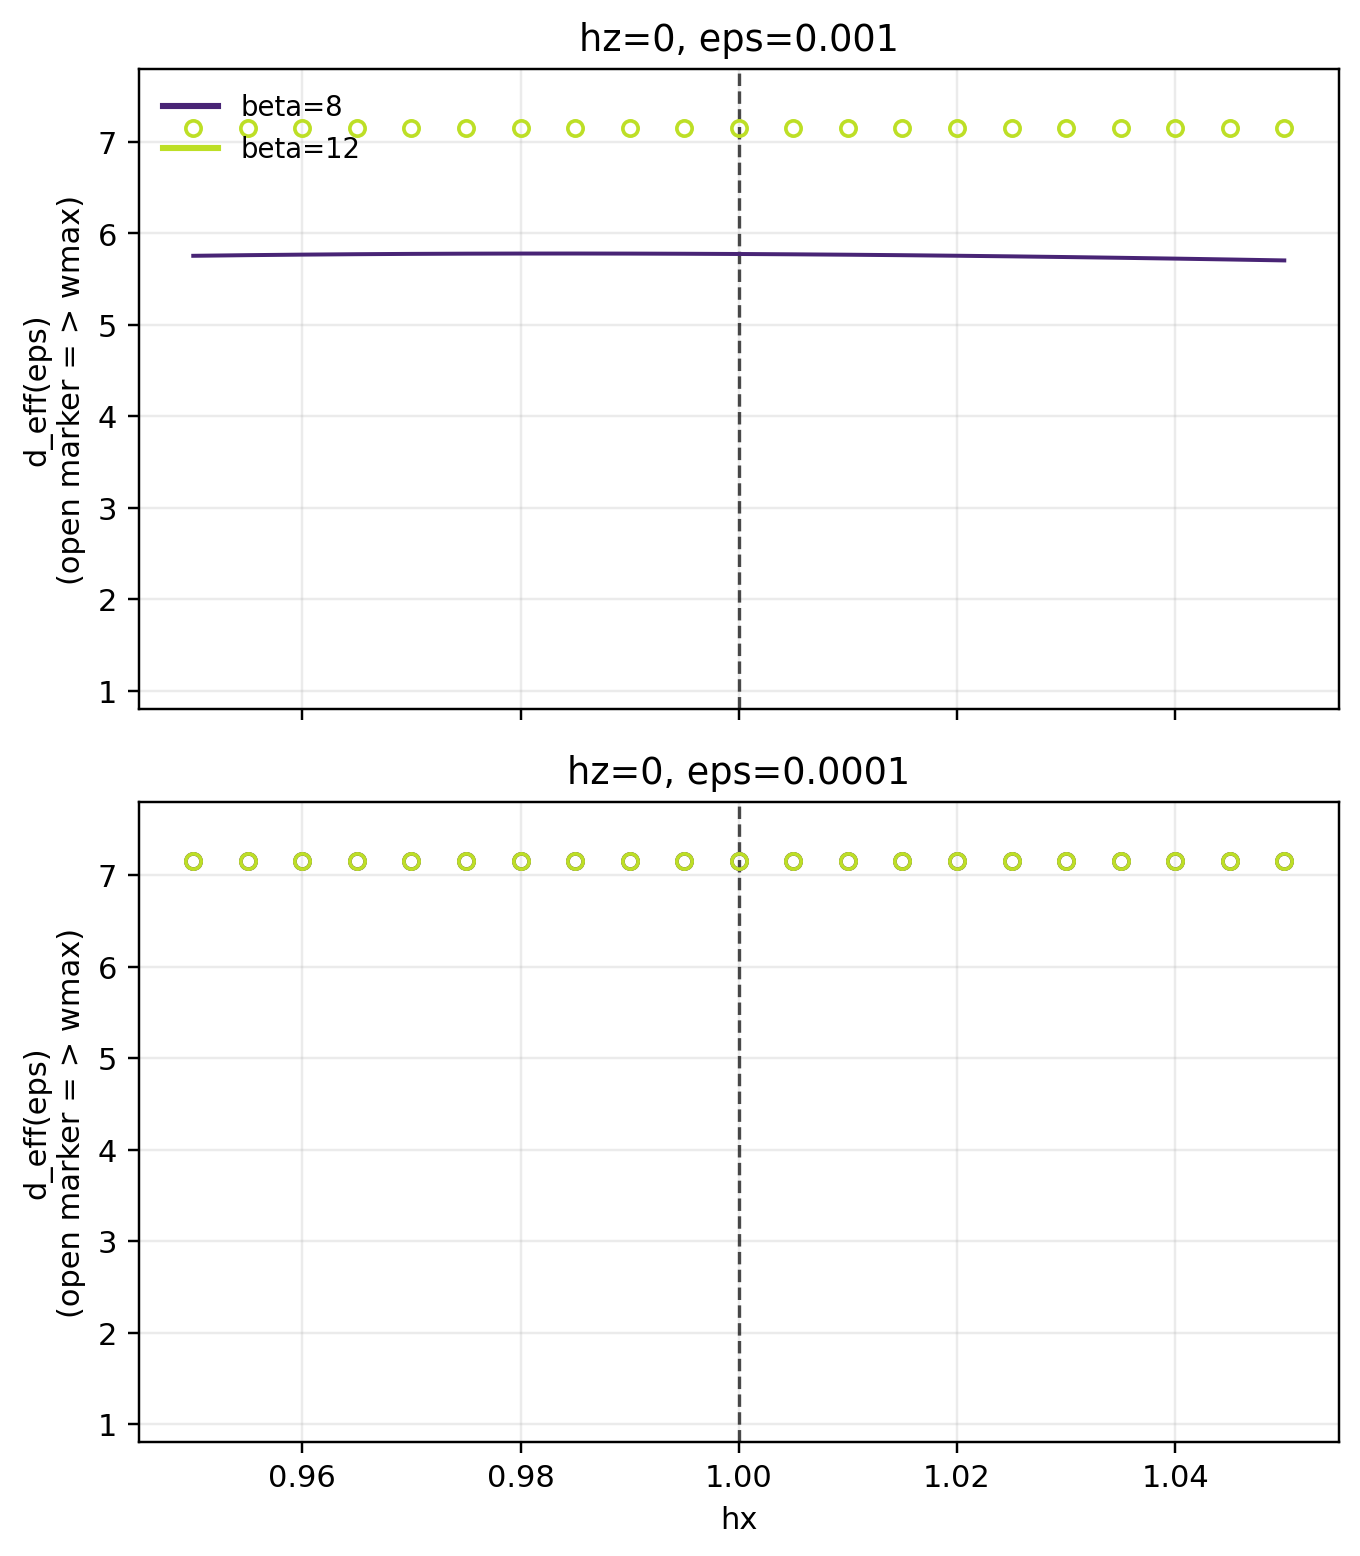
\includegraphics[width=0.7\textwidth]{fig2_zoom.png}
\caption{Zoom sweep at $h_z = 0$, $N = 11$, $\beta \in \{8, 12\}$,
$\varepsilon \in \{10^{-3}, 10^{-4}\}$, $w_{\max} = 7$ (v1 figure,
unchanged).}
\end{figure}

\section{CMI companion diagnostic (added in v2)}
\label{sec:cmi}
v1 listed comparing $\deff$ to CMI-based diagnostics as future work; the
suite delivers it on the same sweep. Define $\deff^{\rm CMI}
(\varepsilon_I)$ by replacing $E_{\rm best}$ with $I_\rho(A:C|B)$ (which
is monotone decreasing in $w$ up to numerical noise). Because CMI decays
about half as fast as the Petz error ($\mu_{\rm Petz} \approx 2\mu_{\rm
CMI}$ in this model family, cf.\ 2601.0035 \cite{S0035}), it needs its
own threshold; choosing the first $\varepsilon_I$ that resolves both
off-critical endpoints ($\varepsilon_I = 3\times 10^{-2}$ at $N = 9$,
$\beta = 12$) gives $\deff^{\rm CMI} = 3, {>}5, {>}5, {>}5, 4, 3$ across
$h_x = 0.7, \dots, 1.3$ at $h_z = 0$ -- the same signature as the Petz
distance, if anything sharper -- with the $h_z = 0.5$ control flat at
$1$. The criticality signature is thus not an artifact of the Petz
construction: it is visible directly in the information-theoretic
quantity that upper-bounds optimal recovery.

\section{Verification suite (added in v2)}
\texttt{verification/2601-0038/verify\_2601\_0038.py} regenerates the
pipeline from scratch (ED; default $N = 9$, \texttt{--N11} for the paper
size; chunked with a JSON cache for constrained environments): the Petz
criticality signature at its resolvable window (Remark~\ref{rem:window}),
the flat control, the CMI companion signature (Section~\ref{sec:cmi}),
the $\beta = 4$ attenuation, the all-censored $\beta = 12$,
$\varepsilon = 10^{-3}$ window, $|C|$ per $w$ reported explicitly, and
monotonicity of $E_{\rm best}$.

\section{Discussion and outlook}
At finite size and temperature the TFIM critical point manifests as a
broadened crossover; the recovery distance $\deff$ grows and censors
there while the perturbed control stays featureless, and the same
signature appears in the CMI diagnostic. Future work: fixed-$|C|$
protocols (growing $N$ with $w$, addressing Remark~\ref{rem:cshrink}),
finite-size scaling in $N$, tensor-network extension of the collar
window.

\section*{Note added in v2}
No v1 result is changed: all figures, tables and numbers stand. v2 adds
what a careful reader needs to weigh them: (1) the $|C|$-shrinkage caveat
(Remark~\ref{rem:cshrink}) qualifying the absolute ``$\approx 8$ sites''
reading while leaving the signature intact; (2) the window-relativity
remark (Remark~\ref{rem:window}), grounded in the regenerated $N = 9$
benchmark; (3) the CMI companion diagnostic (Section~\ref{sec:cmi}),
delivering v1's future-work item and showing the signature is not
Petz-specific; (4) series positioning (v1 cited no companion papers) and
a fully regenerable verification suite.

\begin{thebibliography}{8}
\bibitem{Petz} D. Petz, Commun. Math. Phys. \textbf{105} (1986) 123--131.
\bibitem{Sachdev} S. Sachdev, \emph{Quantum Phase Transitions}, 2nd ed.,
Cambridge University Press (2011).
\bibitem{S0035} L. Eriksson, ai.viXra:2601.0035 (2026; v2 2026).
\bibitem{S0101} L. Eriksson, ai.viXra:2512.0101 (2025; v2 2026).
\bibitem{S0060} L. Eriksson, ai.viXra:2512.0060 (2025; v2 2026).
\bibitem{S0034} L. Eriksson, ai.viXra:2601.0034 (2026; v2 2026).
\end{thebibliography}
\end{document}
